\documentclass{article}

% Language setting
% Replace `english' with e.g. `spanish' to change the document language
\usepackage[english]{babel}

% Set page size and margins
% Replace `letterpaper' with `a4paper' for UK/EU standard size
\usepackage[letterpaper,top=2cm,bottom=2cm,left=3cm,right=3cm,marginparwidth=1.75cm]{geometry}

% Useful packages
\usepackage{amsmath}
\usepackage{graphicx}
\usepackage[colorlinks=true, allcolors=blue]{hyperref}

\title{Your Paper}
\author{Nuno Pires}

\begin{document}
\maketitle

\begin{abstract}
Your abstract.
\end{abstract}

\section{Data Sources}
\begin{itemize}
    \item Variety of Portugal GIS datasets from the Linking Landscape, Environment, Agriculture and Food - Green and Blue Infrastructures", Instituto Superior de Agronomia and other sources. Shapefiles or geoTiff in EPSG:3763, ETRS89/Portugal TM06, metadata in xml format, layout and a map preview. \url{http://epic-webgis-portugal.isa.ulisboa.pt/data#relevo}
    \item Geocatalogo - Catálogo com informação geográfica de dados abertos (opendata) disponível para descarregar em diversos formatos \url{https://geocatalogo.icnf.pt/catalogo_tema2.html}
    \item \url{https://github.com/centraldedados/incendios/tree/master}
\end{itemize}

\section{Questões}
\begin{enumerate}
\item Fuel moisture is a measure of the amount of water in a fuel (vegetation) available to a fire; O artigo X, cita o fator de fuel moisture como um o principal parâmetro de ignição de fogo florestal. 
\item and like this.
\end{enumerate}
\dots or bullet points \dots
\begin{itemize}
\item Like this,
\item and like this.
\end{itemize}

\section{Mapping Forest Fire Risk—A Case Study in
Galicia (Spain) \cite{Novo2020MappingFF}}

\subsection{Fatores que Contribuem para o ínicio de um incêndio, e propagação}
\begin{enumerate}
\item topografia (elevação, e inclinação)
\item vegetação
\item meteorologia
\item fatores humanos
\item distância a estradas
\item distância a povoações
\end{enumerate}

\subsection{Tipos de Risco}
\begin{enumerate}
\item Risco a longo prazo: define-se pelas componentes de um território que não variam a longo prazo como a topografia, e o tipo de vegetação.
\item Risco a curto prazo: definese pelo for fatores que mudam, como as condições do clima.
\end{enumerate}
Risco de Incêncido define-se como a probabilidade de de ocorrência de um fogo florestal, e o dano, que potencialmente, pode vir a causar num lugar(Vulnerabilidade).
Três categorias de controlo de incêndio: Predição, monitoramento, e predição.

\subsection{Fire Weather Index} 
Componente do sistema canadiano de classificação do perigo de incêndio florestal. Neste artigo, foi usado para avaliar o perigo de incêndio, que tem em conta os efeitos da humidade do combustível.

\begin{enumerate}
    \item Temperatura (◦C)
    \item Direção do Vento(◦)
    \item Velocidade do Vento(km/h)
    \item Humidade relativa(%)
    \item Pressão absoluta(hPa)
    \item Chuva instantânea (mm)
    \item Precipitação acumulada nas últimas 24h
\end{enumerate}

\subsection{Problemas Antropogénicos}
Atividades humanas estão associadas com a ocorrência de fogo florestal, e a proximidade com as áreas urbanas, e estradas.


\section{To Predict the Fire Outbreak in Australia using 
Historical Database \cite{9964603}}
A Machine Learning based Decision Tree
Model to construct a Forest Fire Prediction Model using data
from the last 20 years from NASA'S FIRMS (Fire Information for Resource Management System) satellite data, on NASA MODIS and VIIRS dataset.
Wildfires produce fine particle air pollution, which directly
threatens human health even during relatively short
exposures.
Extreme fire occurrences had accounted for 25% of all
fire incidents with the Northern Territory experiencing the
maximum number of fire incidents. It was noted that
Grasslands and Forests were more susceptible to fire than
other types of vegetation.
Tropical zones had the maximum number of fire
occurrences in a week (967), an almost periodic seasonal
frequency pattern. Grasslands had the highest weekly
frequency (1067).


Forest fire data from the Montesinho 
natural park in Portugal’s Tras-os-Montes upper east zone, 
collected over three years

Weather forecasting is used to 
predict the favorable climatic conditions for forest fires to 
take measures accordingly for that particular day

\section{Environmental Fire Hazard Detection and 
Prediction using Random Forest Algorithm \cite{9726029}}
X x-axis spatial coordinate within the Montesinho park map: 1 to 9
Y y-axis spatial coordinate within the Montesinho park map: 2 to 9
Month Month of the year: ‘Jan’ to ‘Dec’
Day Day of the week: ‘Mon’ to ‘Sun’
FFMC Fine Fuel Moisture Code (FFMC) index from the Fire Weather 
Index (FWI) system: 18.7 to 96.20
DMC Duff Moisture Code (DMC) index from the FWI system: 1.1 to 
291.3
DC Drought Code (DC) index from the FWI system: 7.9 to 860.6
ISI Initial Spread Index (ISI) index from the FWI system: 0.0 to 
56.10
Temp Temperature in Celsius degrees: 2.2 to 33.30
RH Relative humidity in %: 15.0 to 100
Wind Wind speed in km/h: 0.40 to 9.40
Rain Outside rain in mm/m2 : 0.0 to 6.4
Area Burned area of the forest (in ha): 0.00 to 1090.84

\begin{figure}[ht]
 \centering
  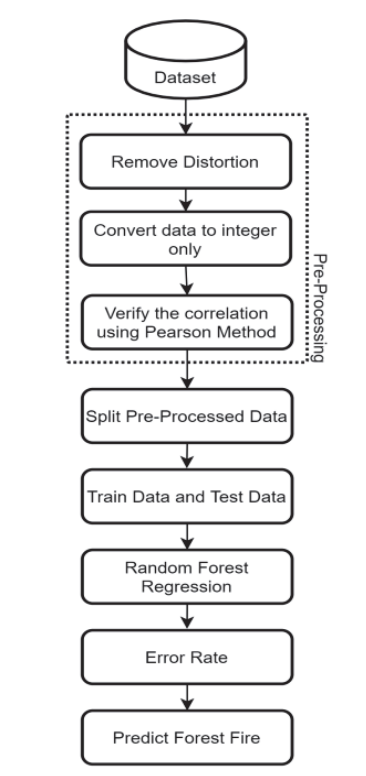
\includegraphics[width=0.25\linewidth]{imgs/flow_chart_detect_fire.png}
   \caption{\label{fig:flow_chaft}This frog was uploaded via the file-tree menu.}
\end{figure}

\begin{figure}[ht]
 \centering
  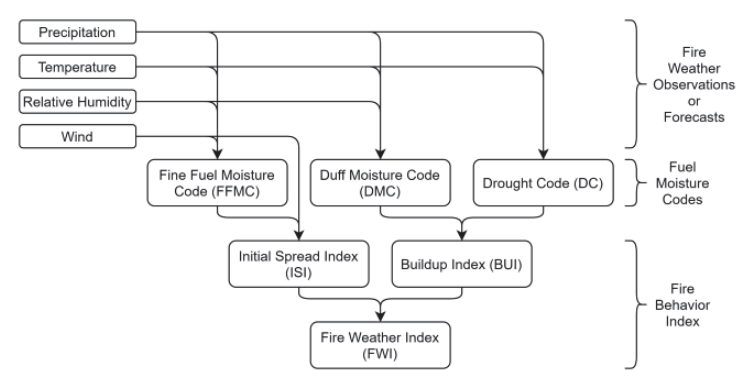
\includegraphics[width=0.70\linewidth]{imgs/fwi_structure.png}
   \caption{\label{fig:fwi_structure}This frog was uploaded via the file-tree menu.}
\end{figure}



1. Temperature is directly related or proportional to 
month, FFMC, DMC, DC, and ISI. 
2. Rain and temperature show the absence of a 
correlation between them. 
3. Rain and FFMC also show the absence of a 
correlation between them. 
4. DC and month have a strong relationship. 

A chuva não tem uma correlação muito forte com as outras variáveis.

The Random Forest regression means the absolute error 
is 0.6664, and the Random forest regression score is 0.9799.



\section{Forest Fire Probability Prediction based on Humidity and Temperature \cite{10085661}}
Este artigo focava na humidade, oxigénio, e temperatura para a previsão. Foi criada uma aplicação onde se inseria estes três valores, e o depois, mostrado a probabilidade de ocorrer um incêndio.   
\subsection{Methodology - Passos para a previsão}
\begin{enumerate}
\item Acquisition of Dataset
\item Data preprocessing: Data Cleaning - Remove any missing or irrelevant data and ensure that the data is in a consistent format, Data Normalization - Normalize the data to ensure that all the variables have similar scales and ranges, Data Splitting - Split the data into training and testing sets to ensure that the model is trained and evaluated on different data and Data Transformation - Transform the data into a format suitable for modeling, such as converting categorical variables into numerical ones.
\item Feature Extraction: Extract relevant features such as average temperature, average humidity, and others to build a predictive model.
\item Building the model: split the data into training and testing sets. Choose an appropriate machine learning
algorithm for the prediction of forest fire probability.
\item Validation and testing
\end{enumerate}

\subsection{Vantagens de Implementação do sistema}
\begin{enumerate}
    \item Improved Accuracy: The use of machine learning algorithms allows the system to make more accurate predictions based on historical data.
    \item Early Warning: The system provides early warning of potential forest fires, allowing authorities to take preventive measures to reduce the risk of fire.
    \item Real-Time Predictions: The system provides real-time predictions based on current temperature and humidity values, which is critical in the prediction of forest fires.
    \item Cost-Effective: The proposed system is cost-effective compared to traditional methods of monitoring and predicting forest fires, which often rely on manual labor.
    \item Automated: The system is automated, reducing the need for manual intervention and increasing efficiency.
    \item Data-Driven: The system is data-driven, allowing for continuous improvement of the predictive model based on new data.
\end{enumerate}

\subsection{Conclusões}
\begin{enumerate}
    \item Muita humidade e baixas temperaturas estão a associadas a uma baixa probabilidade de ocorrência de incêndio.
    \item O uso de apenas três variáveis não é suficiente para prever fogo florestal, é necessário conjugar com a velocidade do vento, topografia, e tipo de vegetação.
\end{enumerate}


\section{Optimization of Geographic Information Systems 
for Forest Fire Risk Assessment \cite{9167162}}
The performed geographic information systems optimization enables easier and faster forecasting of critical points that could be threatened by fire
\begin{enumerate}
    \item Creating thematic layers - represent land use, population density, vegetation types, elevation, etc.
    \item Spatial analysis (understanding the relationships between geographic features or datasets) and creation of thematic maps.
    \item Development of a digital terrain model and analysis of orographic (study of the topographic relief of mountains) features relevant to the rate and direction of fire.
    \item Analysis of matrix substrate and soil type.
    \item Analysis of socio-demographic traits.
spread;
\end{enumerate}


\section{A smart approach for fire prediction under uncertain
conditions using machine learning \cite{Sharma2020}}
Estudo realizado num dataset que continha 517 instâncias e 13 atributos, mas apenas 2 atributos, temperatura e humidade relativa foram considerados.

\begin{figure}[ht]
 \centering
  \includegraphics[width=0.80\linewidth]{imgs/tabela_resultados_previsão.png}
   \caption{\label{fig:flow_chaft}Comparação entre os 8 modelos}
\end{figure}

O AUC demonstra o a efetividade de um modelo para distinguir entre casos correspondentes a fogo, e a casos sem fogo. Quanto maior o AUC, melhor é o modelo a fazer a distinção.





























































\subsection{How to create Sections and Subsections}

Simply use the section and subsection commands, as in this example document! With Overleaf, all the formatting and numbering is handled automatically according to the template you've chosen. If you're using the Visual Editor, you can also create new section and subsections via the buttons in the editor toolbar.

\subsection{How to include Figures}

First you have to upload the image file from your computer using the upload link in the file-tree menu. Then use the includegraphics command to include it in your document. Use the figure environment and the caption command to add a number and a caption to your figure. See the code for Figure \ref{fig:frog} in this section for an example.

Note that your figure will automatically be placed in the most appropriate place for it, given the surrounding text and taking into account other figures or tables that may be close by. You can find out more about adding images to your documents in this help article on \href{https://www.overleaf.com/learn/how-to/Including_images_on_Overleaf}{including images on Overleaf}.

\begin{figure}
\centering
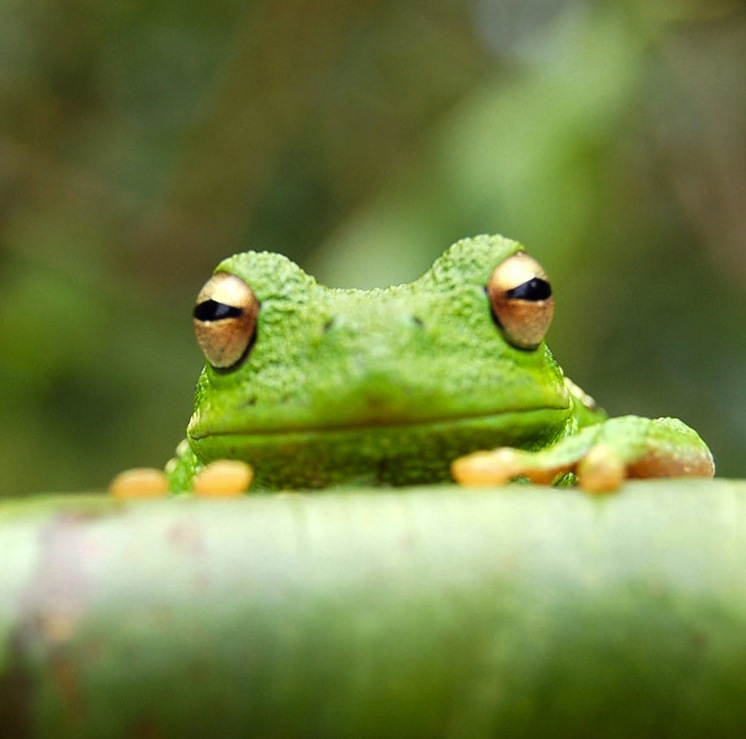
\includegraphics[width=0.25\linewidth]{frog.jpg}
\caption{\label{fig:frog}This frog was uploaded via the file-tree menu.}
\end{figure}

\subsection{How to add Tables}

Use the table and tabular environments for basic tables --- see Table~\ref{tab:widgets}, for example. For more information, please see this help article on \href{https://www.overleaf.com/learn/latex/tables}{tables}. 

\begin{table}
\centering
\begin{tabular}{l|r}
Item & Quantity \\\hline
Widgets & 42 \\
Gadgets & 13
\end{tabular}
\caption{\label{tab:widgets}An example table.}
\end{table}

\subsection{How to add Comments and Track Changes}

Comments can be added to your project by highlighting some text and clicking ``Add comment'' in the top right of the editor pane. To view existing comments, click on the Review menu in the toolbar above. To reply to a comment, click on the Reply button in the lower right corner of the comment. You can close the Review pane by clicking its name on the toolbar when you're done reviewing for the time being.

Track changes are available on all our \href{https://www.overleaf.com/user/subscription/plans}{premium plans}, and can be toggled on or off using the option at the top of the Review pane. Track changes allow you to keep track of every change made to the document, along with the person making the change. 

\subsection{How to add Lists}

You can make lists with automatic numbering \dots



\subsection{How to write Mathematics}

\LaTeX{} is great at typesetting mathematics. Let $X_1, X_2, \ldots, X_n$ be a sequence of independent and identically distributed random variables with $\text{E}[X_i] = \mu$ and $\text{Var}[X_i] = \sigma^2 < \infty$, and let
\[S_n = \frac{X_1 + X_2 + \cdots + X_n}{n}
      = \frac{1}{n}\sum_{i}^{n} X_i\]
denote their mean. Then as $n$ approaches infinity, the random variables $\sqrt{n}(S_n - \mu)$ converge in distribution to a normal $\mathcal{N}(0, \sigma^2)$.


\subsection{How to change the margins and paper size}

Usually the template you're using will have the page margins and paper size set correctly for that use-case. For example, if you're using a journal article template provided by the journal publisher, that template will be formatted according to their requirements. In these cases, it's best not to alter the margins directly.

If however you're using a more general template, such as this one, and would like to alter the margins, a common way to do so is via the geometry package. You can find the geometry package loaded in the preamble at the top of this example file, and if you'd like to learn more about how to adjust the settings, please visit this help article on \href{https://www.overleaf.com/learn/latex/page_size_and_margins}{page size and margins}.

\subsection{How to change the document language and spell check settings}

Overleaf supports many different languages, including multiple different languages within one document. 

To configure the document language, simply edit the option provided to the babel package in the preamble at the top of this example project. To learn more about the different options, please visit this help article on \href{https://www.overleaf.com/learn/latex/International_language_support}{international language support}.

To change the spell check language, simply open the Overleaf menu at the top left of the editor window, scroll down to the spell check setting, and adjust accordingly.

\subsection{How to add Citations and a References List}

You can simply upload a \verb|.bib| file containing your BibTeX entries, created with a tool such as JabRef. You can then cite entries from it, like this: \cite{greenwade93}. Just remember to specify a bibliography style, as well as the filename of the \verb|.bib|. You can find a \href{https://www.overleaf.com/help/97-how-to-include-a-bibliography-using-bibtex}{video tutorial here} to learn more about BibTeX.

If you have an \href{https://www.overleaf.com/user/subscription/plans}{upgraded account}, you can also import your Mendeley or Zotero library directly as a \verb|.bib| file, via the upload menu in the file-tree.

\subsection{Good luck!}

We hope you find Overleaf useful, and do take a look at our \href{https://www.overleaf.com/learn}{help library} for more tutorials and user guides! Please also let us know if you have any feedback using the Contact Us link at the bottom of the Overleaf menu --- or use the contact form at \url{https://www.overleaf.com/contact}.

\bibliographystyle{plain}
\bibliography{referencias}

\end{document}